\chapter{Fundamentação Teórica}

\section{Jogos Interativos por Computador}

Alguns dos efeitos negativos dos jogos por computador podem ser resolvidos
incorporando nos jogos interações como movimentos físicos como mecanismo de
controle, em um caso mais promissor, o principio de imersão no jogo, de forma que
o usuário possa interagir, como se ele mesmo estivesse dentro, com os outros
elementos.Para isso será necessário módulo de captura de movimento da imagem do
usuário, detecção e sequenciamento de parte do corpo que transmite a informação
de controle, análise de informação, tradução para transformar em controle e
ativação de algum elemento no jogo.

\subsection{Jogos por computador}

Um jogo é uma atividade composta por uma série de ações e decisões, limitado por
regras e por um ambiente virtual, que resultam em um condição final.
Essas regras e ambiente são controlados por um programa digital e existem para
proporcionar uma estrutura e um contexto para as ações do jogador, as regras
não devem ser ambíguas e tem como objetivo criar desafios e se contrapor ao
jogador.Em todo instante existe situações opcionais e negociação por
alternativas, as diferentes condições finais são atribuídos diferentes valores,
o jogador executa as ações de forma a influenciar a condição final.\cite{DesignGames}

\subsection{Interatividade e Imersividade em jogos}

\section{Processamento das Imagens e Rastreamento de movimento}

Quando estamos lidando com vídeos, ao invés de apenas alguma imagem,
frequentemente estamos interessados em seguir um objeto em particular
dentro do campo de visão, a identificação deve se dar de um quadro para
o próximo quadro do vídeo. Existem diversos algoritmos e técnicas.

\subsection{Rastreamento por cor}

Se um dado objeto que estamos interessados em rastrear tem uma cor única dentro
do campos de visão da câmera, é possível aplicarmos uma máscara que irá subtrair
de cada frame todos os pixels que não estiverem dentro de uma variação escolhida.
O resultado será uma imagem onde todos os pixels que forem da cor selecionada
serão brancos e os demais serão pretos.

\subsection{Rastreamento por detecção baseada em características do tipo Haar}

Em uma imagem,  uma característica de dois retângulos é a diferença  entre a soma
dos pixels de dois retângulos adjacentes. Uma característica de três retângulos
considera três retângulo adjacentes e é a diferença entre a soma dos pixels dos
dois retângulos extremos e do retângulo do meio. Uma característica de quatro
retângulos considera quatro retângulos dispostos na forma 2 x 2 e é a diferença
entre a soma dos pixels dos dois retângulos da diagonal principal e a soma dos
pixels dos dois retângulos da outra diagonal. Estas características são chamadas
de características do tipo Haar.

Esse método serve para detecção de objetos rígidos em uma determinada perspectiva.
Como o classificador é treinado para um banco de imagens, é possível treiná-lo
para detectar por exemplo olho, nariz, face, mão , corpo inteiro,etc

\begin{figure}[h]
    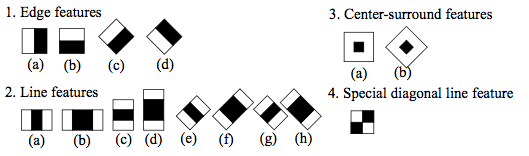
\includegraphics[scale=0.90]{imagens/haarfeatures.png}

    \caption{Características do tipo Haar}
    \label{haarfeatures}
\end{figure}

\subsection{Convex Hull}

